\chapter{Definition von Turbo Codes}
% ----------------------------

\autoref{fig:Codierungsgewinn in der Satellitenkommunikation} beschreibt die Turbocodierung, annhand vier Turbocodes, mit  satelliten Kommunikationspaketen. Der Wert von \(m\) ist die Nachrichtenlänge.\cite[S. 7]{huffman}

\begin{figure}[!ht]
    \centering
     {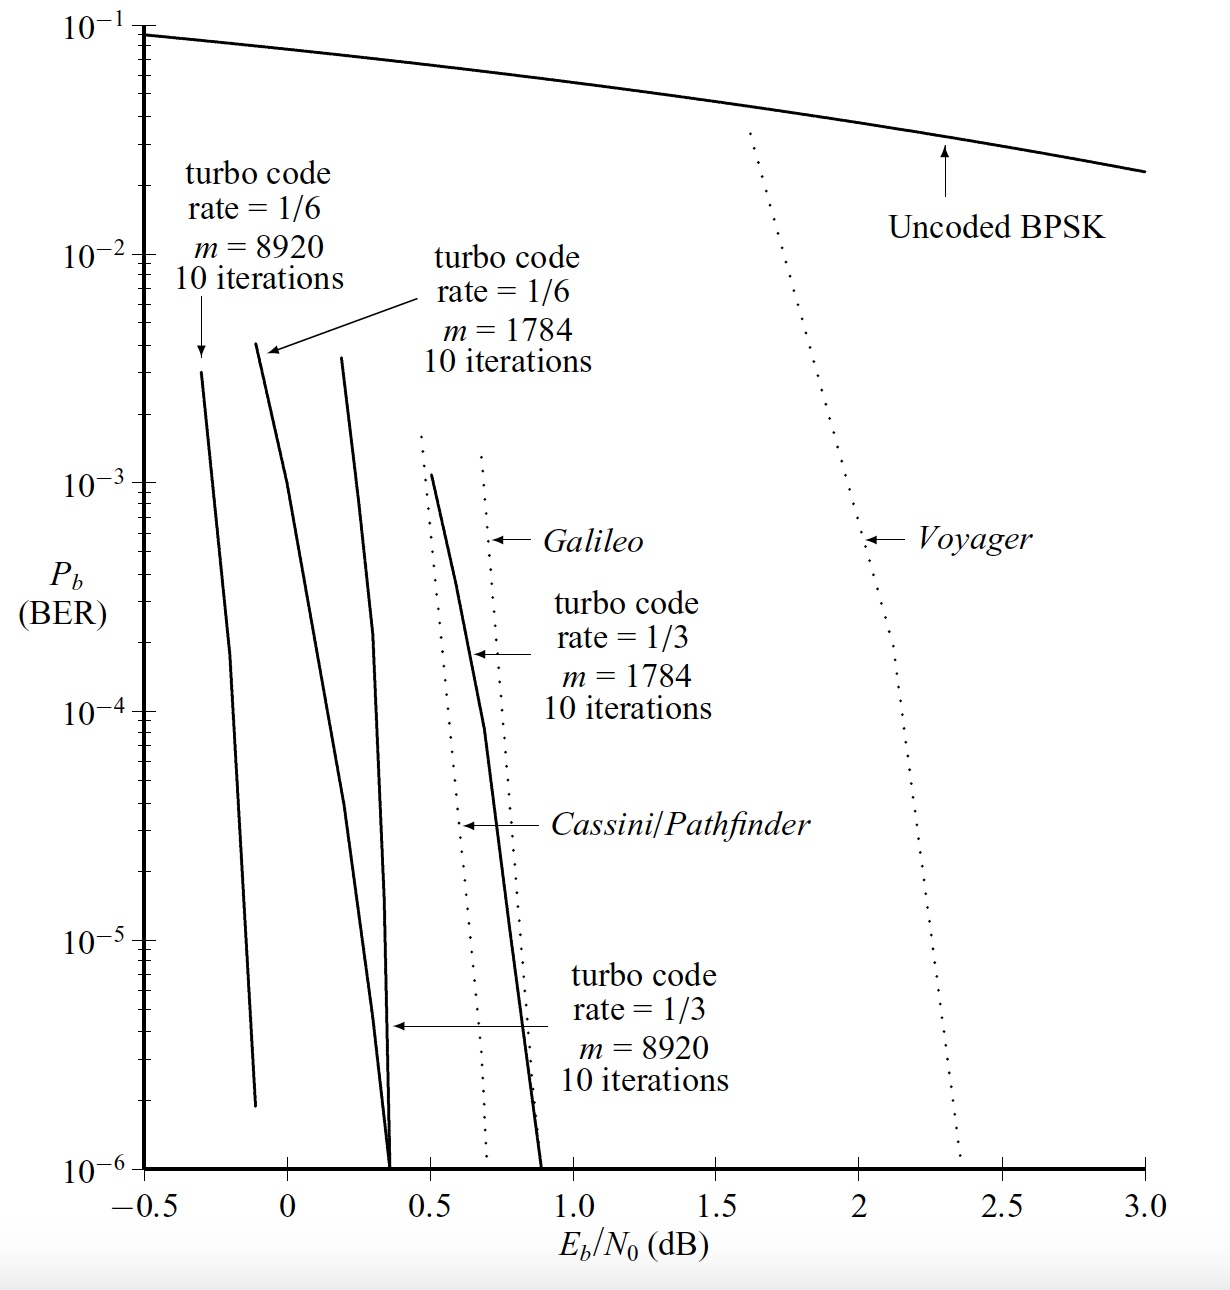
\includegraphics[width=0.7\textwidth]{./pic/Codierungsgewinn in der Satellitenkommunikation}}
    \caption{ Codierungsgewinn in der Satellitenkommunikation}
    \label{fig:Codierungsgewinn in der Satellitenkommunikation}
\end{figure} 
\autoref{fig:Codierungsgewinn in der Satellitenkommunikation}

In \autoref{fig:kommunikationskanal}
wird gezeigt, 
dass ein Ziel der Kodierung darin besteht, mit Signal-Rausch-Verhältnissen nahe der 
Shannon-Grenze zu kommunizieren. 
\autoref{fig:Codierungsgewinn in der Satellitenkommunikation}
zeigt den Vergleich zwischen dem Signal-Rausch-Verhältnis 
Eb/N0 und der Bitfehlerrate Pb der in einigen Satelliten Kommunikationspaketen 
verwendeten Codes.
\pagebreak

\begin{definition}[parallel verketteter Code]
Ein parallel verketteter Code besteht aus zwei oder mehr Komponenten-Codes, 
bei denen es sich in der Regel entweder um 
binäre Faltungscodes oder um Blockcodes mit einer Trellis-Struktur handelt, 
die zu einer effizienten Dekodierung mit weichen Entscheidungen führt.\\

Wenn die
Komponentencodes des parallel verketteten Codes faltbar sind, wird der resultierende Code als parallel
verketteter Faltungscode oder PCCC bezeichnet. Der Komponentencode hat die Coderate $1/2$, da jedes Nachrichtenbit zwei Codewortbits erzeugt.\\

Im einfachsten Fall, 
handelt es sich um zwei Komponenten-Codes, $C_1$ und $C_2$, 
mit jeweils systematischen Kodierern. Tatsächlich können die Kodierer 
für die beiden Codes identisch sein. \cite[S. 8]{huffman}
\\ 
\end{definition}


\begin{Beispiel}[parallel verketteter Code]
Angenommen, es Existieren Komponentencodes $C_i$ zu einem $[n, n/2]$ Binär-
blockcode mit der Generatormatrix $G_i$ = $[I_{n/2} \quad A_{i}]$, die als Kodierer bezeichnet werden.\\

Bei der vorgehnsweise wendet man die übliche Kodierung an, bei der die Nachricht mit
$xG_i$ kodiert wird. Ein Kodierer für den parallel-verketteten Code mit den Komponenten-Kodierern $xG_1$ und $xG_2$
wird wie folgt gebildet.\\

Die Nachricht $x$ wird mit dem ersten Code kodiert, um $(x, c_1)$ zu erzeugen, wobei $c_1 = xG_1$ ist, wenn der Code ein Blockcode ist. Als nächstes wird die Nachricht $x$ an einen Permuter, auch Interleaver genannt,
weitergeleitet. Der Permuter wendet eine feste Permutation auf die Koordinaten von $x$ an und erzeugt die permutierte Nachricht $\bar{x}$. Die permutierte Nachricht $\bar{x}$ wird mit $G_2$ kodiert, um $(\bar{x}, c_2)$ zu erzeugen, wobei $c_2 = \bar{x}G_2$.\\

Das Codewort, dass an den Kanal weitergegeben wird, ist eine verschachtelte Version der ursprünglichen Nachricht $x$ und der beiden Redundanzzeichenfolgen $c_1$ und $c_2$, die durch die Codes $C_1$ und $C_2$ erzeugt
wurden.\\

Dieser Vorgang ist in im nächstes Abschnitt in
\autoref{fig:Parallel verketteter Code mit zwei Komponenten} dargestellt und wird anhand einer mathematischen Aufgabe genauer erläutert.\\
\end{Beispiel}
\pagebreak

% ----------------------------
\section{Beispielmodell: Ein parallel verketteter Code}
% ---------------------------- 

\begin{Beispiel}[parallel verketteter Code]
Seien $C_1$ und $C_2$ jeweils der erweiterte $[8, 4, 4]$ Hamming-Code mit Generatormatrix


$G_{1}=G_2=\left( \begin{array}{rrrrrrrr}
    1 & 0 & 0 & 0 & 0 & 1 & 1 & 1 \\
    0 & 1 & 0 & 0 & 1 & 0 & 1 & 1 \\
    0 & 0 & 1 & 0 & 1 & 1 & 0 & 1 \\
    0 & 0 & 0 & 1 & 1 & 1 & 1 & 0 \\
   \end{array}\right). 
$\\

Angenommen, der Permuter ist durch die Permutation $(1,\quad 3)(2,\quad 4)$ gegeben.

Die zu kodierende Nachricht ist beispielsweise $x = (1,0,1,1).$ Dann ist $xG_1 = (1,0,1,1,0,1,0,0)$ und   $c_1 = (0,1,0,0)$. Die permutierte Nachricht ist $\bar{x} = (1,1,1,0)$, die als $\bar{x}G_2 = (1,1,1,0,0,0,0,1)$ kodiert wird und $c_2 = (0,0,0,1)$ ergibt.


\begin{figure}[!ht]
    \centering
     {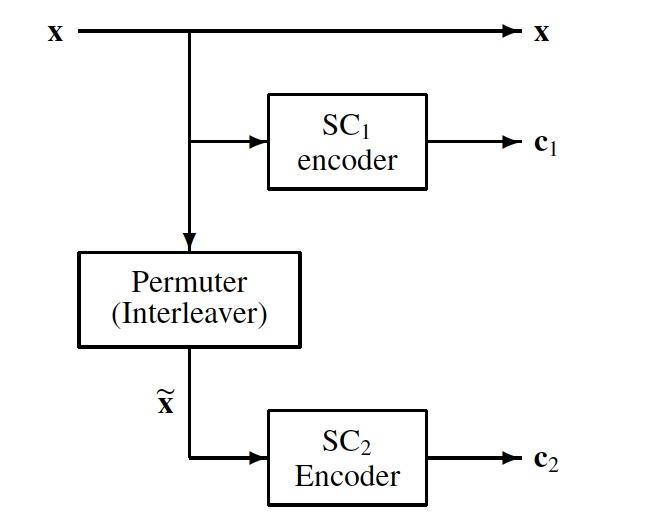
\includegraphics[width=0.7\textwidth]{./pic/Parallel verketteter Code mit zwei Komponenten}}
    \caption{ Parallel verketteter Code mit zwei Komponenten}
    \label{fig:Parallel verketteter Code mit zwei  Komponenten}
\end{figure} 

Dann wird $(x, c_1, c_2) = ((1,0,1,1), (0,1,0,0), (0,0,0,1))$ in verschachtelter Form übertragen, wobei die ersten Bits von $x, c_1, c_2$, gefolgt werden von den zweiten Bits, dritten Bits und vierten Bits, als $((1,0,0), (0,1,0), (1,0,0), (1,0,1)).$\\

In der \autoref{fig:Parallel verketteter Code mit zwei Komponenten} zeigen $SC_1$ und $SC_2$, 
dass die Kodierer in Standardform vorliegen. 
Der resultierende parallel verkettete Code hat die Coderate von $1/3$.
\end{Beispiel} \cite[S. 9]{huffman}
\pagebreak

\begin{Beispiel}[parallel verketteter Code]
    Finde die Permuter Form aller $16$ Codewörter des in Beispielaufgabe $a$ beschriebenen parallel verketteten Codes und bestimme den minimalen Abstand des resultierenden $[12, 4]$ Binärcodes.\\
    
    Um die Aufgabe zu Lösen, geht man schrittweise vor:
    
    Zu einem $[8, 4, 4]$ Hamming-Code findet man alle $2^4 = 16$ empfangenen Nachrichten $x$, da der Code vier Informationsbits aufweist.
    
    Die $16$ möglichen $x$ Nachrichten sind:\\
    
    $x_1= (0,0,0,0)$
    
    $x_2= (0,0,0,1)$
    
    $x_3= (0,0,1,0)$ 
    
    $x_4= (0,1,0,0)$ 
    
    $x_5= (1,0,0,0)$ 
    
    $x_6= (0,0,1,1)$ 
    
    $x_7= (0,1,0,1)$ 
    
    $x_8= (1,0,0,1)$ 
    
    $x_9= (0,1,1,0)$ 
    
    $x_{10}= (1,0,1,0)$ 
    
    $x_{11}= (1,1,0,0)$ 
    
    $x_{12}= (0,1,1,1)$ 
    
    $x_{13}= (1,1,1,0)$ 
    
    $x_{14}= (1,1,0,1)$ 
    
    $x_{15}= (1,0,1,1)$ 
    
    $x_{16}= (1,1,1,1)$\\
    \pagebreak
    
    Durch Multiplikation dieser $16$ Nachricht mit $xG_1$ erhält man die Codewörter $c_1$.\\
    
    $x_1G_1= (0,0,0,0,0,0,0,0) \Rightarrow c_1= (0,0,0,0)$
    
    $x_2G_1= (0,0,0,1,1,1,1,0) \Rightarrow c_1= (1,1,1,0)$
    
    $x_3G_1= (0,0,1,0,1,1,0,1) \Rightarrow c_1= (1,1,0,1)$
    
    $x_4G_1= (0,1,0,0,1,0,1,1) \Rightarrow c_1= (1,0,1,1)$
    
    $x_5G_1= (1,0,0,0,0,1,1,1) \Rightarrow c_1= (0,1,1,1)$
    
    $x_6G_1= (0,0,1,1,2,2,1,1) \bmod 2 = (0,0,1,1,0,0,1,1) \Rightarrow c_1= (0,0,1,1)$
    
    $x_7G_1= (0,1,0,1,2,1,2,1) \bmod 2 = (0,1,0,1,0,1,0,1) \Rightarrow c_1= (0,1,0,1)$
    
    $x_8G_1= (1,0,0,1,1,2,2,1) \bmod 2 = (1,0,0,1,1,0,0,1) \Rightarrow c_1= (1,0,0,1)$
    
    $x_9G_1= (0,1,1,0,2,1,1,2) \bmod 2 = (0,1,1,0,0,1,1,0) \Rightarrow c_1= (0,1,1,0)$
    
    $x_{10}G_1= (1,0,1,0,1,2,1,2) \bmod 2 = (1,0,1,0,1,0,1,0) \Rightarrow c_1= (1,0,1,0)$
    
    $x_{11}G_1= (1,1,0,0,1,1,2,2) \bmod 2 = (1,1,0,0,1,1,0,0) \Rightarrow c_1= (1,1,0,0)$
    
    $x_{12}G_1= (0,1,1,1,3,2,2,2) \bmod 2 = (0,1,1,1,1,0,0,0) \Rightarrow c_1= (1,0,0,0)$
    
    $x_{13}G_1= (1,1,1,0,2,2,2,3) \bmod 2 = (1,1,1,0,0,0,0,1) \Rightarrow c_1= (0,0,0,1)$
    
    $x_{14}G_1= (1,1,0,1,2,2,3,2) \bmod 2 = (1,1,0,1,0,0,1,0) \Rightarrow c_1= (0,0,1,0)$
    
    $x_{15}G_1= (1,0,1,1,2,3,2,2) \bmod 2 = (1,0,1,1,0,1,0,0) \Rightarrow c_1= (0,1,0,0)$
    
    $x_{16}G_1= (1,1,1,1,3,3,3,3) \bmod 2 = (1,1,1,1,1,1,1,1) \Rightarrow c_1= (1,1,1,1)$\\
    
    Die Permutation $(1,\quad 3)(2,\quad 4)$ tauscht die ersten beiden Bits der Nachricht $x$ mit den dritten und vierten Bits.\\
    Angenommen, es existiert eine Nachricht $x$ mit vier Bits $x = (a,b,c,d)$\\
    
    $(1,\quad 3)$: Bit $a$ wird mit dem dritten Bit $c$ getauscht.
    
    $(2,\quad 4)$: Bit $b$ wird mit dem vierten Bit $d$ getauscht.
    
    Dies führt zu einer permutierten neuen Nachricht $\bar{x}=(c,d,a,b).$\\
    
    Die Nachricht $x_1= (0,0,0,0)$ und $x_{16}=(1,1,1,1)$\\ bleiben unverändert, da alle Bits gleich sind.\\
    
    Die Nachricht $x_{15}=(1,0,1,1)$:\\
    Ursprüngliche Form: $(a= 1, b=0, c=1, d=1)$\\
    Nach Permutation: $\bar{x}_{15}=(c,d,a,b)=(1,1,1,0)$\\
    
    Die Nachricht $x_9= (0,1,1,0):$\\
    Ursprüngliche Form: $(a=0, b=1, c=1, d=0)$\\
    Nach Permutation: $\bar{x}_{9}=(c,d,a,b)=(1,0,0,1)$\\
    \pagebreak

    Angewandt auf alle $16$ möglichen Empfangenen Nachrichten $x$ erhält man:\\
    
    $x_1= (0,0,0,0) \Rightarrow \bar{x}_{1} = (0,0,0,0)$
    
    $x_2= (0,0,0,1) \Rightarrow \bar{x}_{2} = (0,1,0,0)$
    
    $x_3= (0,0,1,0) \Rightarrow \bar{x}_{3} = (1,0,0,0)$
    
    $x_4= (0,1,0,0) \Rightarrow \bar{x}_{4} = (0,0,0,1)$
    
    $x_5= (1,0,0,0) \Rightarrow \bar{x}_{5} = (0,0,1,0)$
    
    $x_6= (0,0,1,1) \Rightarrow \bar{x}_{6} = (1,1,0,0)$
    
    $x_7= (0,1,0,1) \Rightarrow \bar{x}_{7} = (0,1,0,1)$
    
    $x_8= (1,0,0,1) \Rightarrow \bar{x}_{8} = (0,1,1,0)$
    
    $x_9= (0,1,1,0) \Rightarrow \bar{x}_{9} = (1,0,0,1)$
    
    $x_{10}= (1,0,1,0) \Rightarrow \bar{x}_{10} = (1,0,1,0)$
    
    $x_{11}= (1,1,0,0) \Rightarrow \bar{x}_{11} = (0,0,1,1)$
    
    $x_{12}= (0,1,1,1) \Rightarrow \bar{x}_{12} = (1,1,0,1)$
    
    $x_{13}= (1,1,1,0) \Rightarrow \bar{x}_{13} = (1,0,1,1)$
    
    $x_{14}= (1,1,0,1) \Rightarrow \bar{x}_{14} = (0,1,1,1)$
    
    $x_{15}= (1,0,1,1) \Rightarrow \bar{x}_{15} = (1,1,1,0)$
    
    $x_{16}= (1,1,1,1) \Rightarrow \bar{x}_{16} = (1,1,1,1)$\\
    
    Durch Multiplikation dieser permutierten Nachrichten mit  $\bar{x}G_2$ erhält man die Codewörter $c_2$:\\
    
    $\bar{x}_{1}G_2= (0,0,0,0,0,0,0,0) \Rightarrow c_2= (0,0,0,0)$
    
    $\bar{x}_{2}G_2= (0,1,0,0,1,0,1,1) \Rightarrow c_2= (1,0,1,1)$
    
    $\bar{x}_{3}G_2= (1,0,0,0,0,1,1,1) \Rightarrow c_2= (0,1,1,1)$
    
    $\bar{x}_{4}G_2= (0,0,0,1,1,1,1,0) \Rightarrow c_2= (1,1,1,0)$
    
    $\bar{x}_{5}G_2= (0,0,1,0,1,1,0,1) \Rightarrow c_2= (1,1,0,1)$
    
    $\bar{x}_{6}G_2= (1,1,0,0,1,1,2,2) \bmod 2 = (1,1,0,0,1,1,0,0) \Rightarrow c_2= (1,1,0,0)$
    
    $\bar{x}_{7}G_2= (0,1,0,1,2,1,2,1) \bmod 2 = (0,1,0,1,0,1,0,1) \Rightarrow c_2= (0,1,0,1)$
    
    $\bar{x}_{8}G_2= (0,1,1,0,2,1,1,2) \bmod 2 = (0,1,1,0,0,1,1,0) \Rightarrow c_2= (0,1,1,0)$
    
    $\bar{x}_{9}G_2= (1,0,0,1,1,2,2,1) \bmod 2 = (1,0,0,1,1,0,0,1) \Rightarrow c_2= (1,0,0,1)$
    
    $\bar{x}_{10}G_2= (1,0,1,0,1,2,1,2) \bmod 2 = (1,0,1,0,1,0,1,0) \Rightarrow c_2= (1,0,1,0)$
    
    $\bar{x}_{11}G_2= (0,0,1,1,2,2,1,1) \bmod 2 = (0,0,1,1,0,0,1,1) \Rightarrow c_2= (0,0,1,1)$
    
    $\bar{x}_{12}G_2= (1,1,0,1,2,2,3,2) \bmod 2 = (1,1,0,1,0,0,1,0) \Rightarrow c_2= (0,0,1,0)$
    
    $\bar{x}_{13}G_2= (1,0,1,1,2,3,2,2) \bmod 2 = (1,0,1,1,0,1,0,0) \Rightarrow c_2= (0,1,0,0)$
    
    $\bar{x}_{14}G_2= (0,1,1,1,3,2,2,2) \bmod 2 = (0,1,1,1,1,0,0,0) \Rightarrow c_2= (1,0,0,0)$
    
    $\bar{x}_{15}G_2= (1,1,1,0,2,2,2,3) \bmod 2 = (1,1,1,0,0,0,0,1) \Rightarrow c_2= (0,0,0,1)$
    
    $\bar{x}_{16}G_2= (1,1,1,1,3,3,3,3) \bmod 2 = (1,1,1,1,1,1,1,1) \Rightarrow c_2= (1,1,1,1)$\\
    \pagebreak
    
    Für jede der $16$ Nachrichten $x$ und jedes Paar $(c_1,c_2)$ erhält man die verschachtelte Form $(x,c_1,c_2):$\\
    
    $(x_1, c_1, c_2) = (0,0,0,0, 0,0,0,0, 0,0,0,0)$
    
    
    $(x_2, c_1, c_2) = (0,0,0,1, 1,1,1,0, 1,0,1,1)$
    
    
    $(x_3, c_1, c_2) = (0,0,1,0, 1,1,0,1, 0,1,1,1)$
    
    
    $(x_4, c_1, c_2) = (0,1,0,0, 1,0,1,1, 1,1,1,0)$
    
    
    $(x_5, c_1, c_2) = (1,0,0,0, 0,1,1,1, 1,1,0,1)$
    
    
    $(x_6, c_1, c_2) = (0,0,1,1, 0,0,1,1, 1,1,0,0)$
    
    
    $(x_7, c_1, c_2) = (0,1,0,1, 0,1,0,1, 0,1,0,1)$
    
    
    $(x_8, c_1, c_2) = (1,0,0,1, 1,0,0,1, 0,1,1,0)$
    
    
    $(x_9, c_1, c_2) = (0,1,1,0, 0,1,1,0, 1,0,0,1)$
    
    
    $(x_{10}, c_1, c_2) = (1,0,1,0, 1,0,1,0, 1,0,1,0)$
    
    
    $(x_{11}, c_1, c_2) = (1,1,0,0, 1,1,0,0, 0,0,1,1)$
    
    
    $(x_{12}, c_1, c_2) = (0,1,1,1, 1,0,0,0, 0,0,1,0)$
    
    
    $(x_{13}, c_1, c_2) = (1,1,1,0, 0,0,0,1, 0,1,0,0)$
    
    
    $(x_{14}, c_1, c_2) = (1,1,0,1, 0,0,1,0, 1,0,0,0)$
    
    
    $(x_{15}, c_1, c_2) = (1,0,1,1, 0,1,0,0, 0,0,0,1)$
     
    
    $(x_{16}, c_1, c_2) = (1,1,1,1, 1,1,1,1, 1,1,1,1)$\\
    
    Die verschachtelte Form $(x,c_1,c_2)$ kombiniert einige Bits aus der ursprünglichen Nachricht $x$, den ursprünglichen Codewörtern $c_1$ und den permutierten Codewörtern $c_2$ und ordnet sie wie folgt an, um sie schlie\ss{}lich als neues kodiertes Codewort mit wahrscheinlich unterschiedlichen Bits an denselben Stellen, also mit einen bestimmten Hamming-Abstand, zu übertragen:\\
    
    Ordnungsalgorithmus:\\
    
    $x= (a,b,c,d) \quad c_1= (e,f,g,h) \quad c_2= (i,j,k,l)\quad (x,c_1,c_2)= ((a,b,c,d), (e,f,g,h), (i,j,k,l))$\\
    
    Die erste Anordnung ordnet die ersten Bits von:\\
    $(x,c_1,c_2) = ((a,b,c,d), (e,f,g,h), (i,j,k,l)) = (a,e,i)$\\
    
    Die zweite Anordnung ordnet die zweiten Bits von:\\
    $(x,c_1,c_2) = ((a,b,c,d), (e,f,g,h), (i,j,k,l)) = ((a,e,i), (b,f,j))$\\
    
    Die letzte Anordnung ordnet die dritten und vierten Bits von:\\
    $(x,c_1,c_2) = ((a,b,c,d), (e,f,g,h), (i,j,k,l)) = ((a,e,i), (b,f,j),(c,g,k), (d,h,l))$\\ 
    
    Wendet man diesen Ordnungsalgorithmus auf alle $16$ verschachtelten Formen an erhält man:\\
    
    
    $(x_{1}, c_1, c_2) = ((0,0,0,0), (0,0,0,0), (0,0,0,0)) \Rightarrow$ Ordnungsalgorithmus: $((0,0,0),(0, 0,0),(0,0, 0),(0,0,0))$ mit Abstand $0$.\\
    
    $(x_{2}, c_1, c_2) = ((0,0,0,1), (1,1,1,0), (1,0,1,1)) \Rightarrow$ Ordnungsalgorithmus: $((0,1,1),(0, 1,0),(0,1, 1),(1,0,1))$ mit Abstand $8$.\\
    \pagebreak
    
    $(x_{3}, c_1, c_2) = ((0,0,1,0), (1,1,0,1), (0,1,1,1)) \Rightarrow$ Ordnungsalgorithmus: $((0,1,0),(0, 1,1),(1,0, 1),(0,1,1))$ mit Abstand $6$.\\
    
    $(x_{4}, c_1, c_2) = ((0,1,0,0), (1,0,1,1), (1,1,1,0)) \Rightarrow$ Ordnungsalgorithmus: $((0,1,1),(1, 0,1),(0,1, 1),(0,1,0))$ mit Abstand $6$.\\
    
    $(x_{5}, c_1, c_2) = ((1,0,0,0), (0,1,1,1), (1,1,0,1)) \Rightarrow$ Ordnungsalgorithmus: $((1,0,1),(0, 1,1),(0,1, 0),(0,1,1))$ mit Abstand $6$.\\
    
    $(x_{6}, c_1, c_2) = ((0,0,1,1), (0,0,1,1), (1,1,0,0)) \Rightarrow$ Ordnungsalgorithmus: $((0,0,1),(0, 0,1),(1,1, 0),(1,1,0))$ mit Abstand $4$.\\
    
    $(x_{7}, c_1, c_2) = ((0,1,0,1), (0,1,0,1), (0,1,0,1)) \Rightarrow$ Ordnungsalgorithmus: $((0,0,0),(1, 1,1),(0,0, 0),(1,1,1))$ mit Abstand $4$.\\
    
    $(x_{8}, c_1, c_2) = ((1,0,0,1), (1,0,0,1), (0,1,1,0)) \Rightarrow$ Ordnungsalgorithmus: $((1,1,0),(0, 0,1),(0,0, 1),(1,1,0))$ mit Abstand $6$.\\
    
    $(x_{9}, c_1, c_2) = ((0,1,1,0), (0,1,1,0), (1,0,0,1)) \Rightarrow$ Ordnungsalgorithmus: $((0,0,1),(1, 1,0),(1,1, 0),(0,0,1))$ mit Abstand $6$.\\
    
    $(x_{10}, c_1, c_2) = ((1,0,1,0), (1,0,1,0), (0,1,0,1)) \Rightarrow$ Ordnungsalgorithmus: $((1,1,1),(0, 0,0),(1,1, 1),(0,0,0))$ mit Abstand $4$.\\
    
    $(x_{11}, c_1, c_2) = ((1,1,0,0), (1,1,0,0), (0,0,1,1)) \Rightarrow$ Ordnungsalgorithmus: $((1,1,0),(1, 1,0),(0,0, 1),(0,0,1))$ mit Abstand $4$.\\
    
    $(x_{12}, c_1, c_2) = ((0,1,1,1), (1,0,0,0), (0,0,1,0)) \Rightarrow$ Ordnungsalgorithmus: $((0,1,0),(1, 0,0),(1,0, 1),(1,0,0))$ mit Abstand $6$.\\
    
    $(x_{13}, c_1, c_2) = ((1,1,1,0), (0,0,0,1), (0,1,0,0)) \Rightarrow$ Ordnungsalgorithmus: $((1,0,0),(1, 0,1),(1,0, 0),(0,1,0))$ mit Abstand $8$.\\
    
    $(x_{14}, c_1, c_2) = ((1,1,0,1), (0,0,1,0), (1,0,0,0)) \Rightarrow$ Ordnungsalgorithmus: $((1,0,1),(1, 0,0),(0,1 ,0),(1,0,0))$ mit Abstand $6$.\\
    
    $(x_{15}, c_1, c_2) = ((1,0,1,1), (0,1,0,0), (0,0,0,1)) \Rightarrow$ Ordnungsalgorithmus: $((1,0,0),(0, 1,0),(1,0, 0),(1,0,1))$ mit Abstand $6$.\\
    
    $(x_{16}, c_1, c_2) = ((1,1,1,1), (1,1,1,1), (1,1,1,1)) \Rightarrow$ Ordnungsalgorithmus: $((1,1,1),(1, 1,1),(1,1, 1),(1,1,1))$ mit Abstand $6$.\\
    
    
    
    
    
    Um den minimalen Abstand genau zu berechnen, müssten man die Hamming-Abstände aller möglichen Paare der $16$ Codewörter bestimmen und den kleinsten Abstand finden. Zwei verschachtelte Codewörter $(x_{1}, c_1, c_2) = ((0,0,0,0), (0,0,0,0), (0,0,0,0))$ und $(x_{16}, c_1, c_2) = ((1,1,1,1), (1,1,1,1), (1,1,1,1))$ sind nach dem Ordnungsalgorithmus identisch, was zu einem Hamming- Abstand von $0$ führt. Demzufolge scheint es so, dass der Mindestabstand des Codes $[12, 4]$ gleich $0$ beträgt. Dies würde jedoch bedeuten, dass der Code $[12, 4]$ keine Fehlererkennung bietet. Dementsprechend beträgt der minimale Abstand des ursprünglichen Codes $[12, 4]$ gleich $4$.\\
    \pagebreak
    
    Die folgenden verschachtelten Codewörtern weisen den minimalen Hamming-Abstand von $4$ auf und werden erfolgreich übertragen.\\
    
    $(x_{6}, c_1, c_2) = ((0,0,1,1), (0,0,1,1), (1,1,0,0)) \Rightarrow$ Ordnungsalgorithmus: $((0,0,1),(0, 0,1),(1,1, 0),(1,1,0))$ mit Abstand $4$.\\
    
    $(x_{7}, c_1, c_2) = ((0,1,0,1), (0,1,0,1), (0,1,0,1)) \Rightarrow$ Ordnungsalgorithmus: $((0,0,0),(1, 1,1),(0,0, 0),(1,1,1))$ mit Abstand $4$.\\
    
    $(x_{10}, c_1, c_2) = ((1,0,1,0), (1,0,1,0), (0,1,0,1)) \Rightarrow$ Ordnungsalgorithmus: $((1,1,1),(0, 0,0),(1,1, 1),(0,0,0))$ mit Abstand $4$.\\
    
    $(x_{11}, c_1, c_2) = ((1,1,0,0), (1,1,0,0), (0,0,1,1)) \Rightarrow$ Ordnungsalgorithmus: $((1,1,0),(1, 1,0),(0,0, 1),(0,0,1))$ mit Abstand $4$.\\
    
\end{Beispiel}


\begin{Beispiel}[parallel verketteter Code]
    Im folgenden ist der Permuter durch die Permutation $(3,\quad 2)(4,\quad 1)$ gegeben:\\

    Die Permutation $(3,\quad 2)(4,\quad 1)$ tauscht das dritte und zweite Bit der Nachricht $x$ mit den vierten und ersten Bit.\\
    
    Angenommen, eine Nachricht $x$ mit vier Bits $x = (a,b,c,d)$\\
    
    $(3,\quad 2)$ bedeutet: Bit $c$ wird mit dem zweiten Bit $b$ getauscht.\\
    $(4,\quad 1)$ bedeutet: Bit $d$ wird mit dem ersten Bit $a$ getauscht.\\
    
    Dies führt zu einer permutierten neuen Nachricht $\bar{x} = (d,c,b,a).$\\
    Die Nachricht  $x_{1} = (0,0,0,0)$ und  $x_{16} = (1,1,1,1)$  bleiben wie bisher unverändert, da alle Bits gleich sind.\\
    
    
    Die Nachricht $x_{15}=(1,0,1,1)$:\\
    Ursprüngliche Form: $(a= 1, b=0, c=1, d=1)$\\
    Nach Permutation: $\bar{x} = (d,c,b,a)=(1,1,0,1)$\\
    
    Die Nachricht $x_9= (0,1,1,0):$\\
    Ursprüngliche Form: $(a=0, b=1, c=1, d=0)$\\
    Nach Permutation: $\bar{x}_{9}=(d,c,b,a)=(0,1,1,0)$\\
    \pagebreak
    
    Angewandt auf alle $16$ möglichen Empfangenen Nachrichten $x$ erhält man:\\
    
    
    $x_1= (0,0,0,0) \Rightarrow \bar{x}_{1} = (0,0,0,0)$
    
    $x_2= (0,0,0,1) \Rightarrow \bar{x}_{2} = (1,0,0,0)$
    
    $x_3= (0,0,1,0) \Rightarrow \bar{x}_{3} = (0,1,0,0)$
    
    $x_4= (0,1,0,0) \Rightarrow \bar{x}_{4} = (0,0,1,0)$
    
    $x_5= (1,0,0,0) \Rightarrow \bar{x}_{5} = (0,0,0,1)$
    
    $x_6= (0,0,1,1) \Rightarrow \bar{x}_{6} = (1,1,0,0)$
    
    $x_7= (0,1,0,1) \Rightarrow \bar{x}_{7} = (1,0,1,0)$
    
    $x_8= (1,0,0,1) \Rightarrow \bar{x}_{8} = (1,0,0,1)$
    
    $x_9= (0,1,1,0) \Rightarrow \bar{x}_{9} = (0,1,1,0)$
    
    $x_{10}= (1,0,1,0) \Rightarrow \bar{x}_{10} = (0,1,0,1)$
    
    $x_{11}= (1,1,0,0) \Rightarrow \bar{x}_{11} = (0,0,1,1)$
    
    $x_{12}= (0,1,1,1) \Rightarrow \bar{x}_{12} = (1,1,1,0)$
    
    $x_{13}= (1,1,1,0) \Rightarrow \bar{x}_{13} = (0,1,1,1)$
    
    $x_{14}= (1,1,0,1) \Rightarrow \bar{x}_{14} = (1,0,1,1)$
    
    $x_{15}= (1,0,1,1) \Rightarrow \bar{x}_{15} = (1,1,0,1)$
    
    $x_{16}= (1,1,1,1) \Rightarrow \bar{x}_{16} = (1,1,1,1)$\\

    
    Durch Multiplikation dieser permutierten Nachrichten mit  $\bar{x}G_2$ erhält man die Codewörter $c_2$:\\
    
    
    $\bar{x}_{1}G_2= (0,0,0,0,0,0,0,0) \Rightarrow c_2= (0,0,0,0)$
    
    $\bar{x}_{2}G_2= (1,0,0,0,0,1,1,1) \Rightarrow c_2= (0,1,1,1)$
    
    $\bar{x}_{3}G_2= (0,1,0,0,1,0,1,1) \Rightarrow c_2= (1,0,1,1)$
    
    $\bar{x}_{4}G_2= (0,0,1,0,1,1,0,1) \Rightarrow c_2= (1,1,0,1)$
    
    $\bar{x}_{5}G_2= (0,0,0,1,1,1,1,0) \Rightarrow c_2= (1,1,1,0)$
    
    $\bar{x}_{6}G_2= (1,1,0,0,1,1,2,2) \bmod 2 = (1,1,0,0,1,1,0,0) \Rightarrow c_2= (1,1,0,0)$
    
    $\bar{x}_{7}G_2= (1,0,1,0,1,2,1,2) \bmod 2 = (1,0,1,0,1,0,1,0 ) \Rightarrow c_2= (1,0,1,0)$
    
    $\bar{x}_{8}G_2= (1,0,0,1,1,2,2,1) \bmod 2 = (1,0,0,1,1,0,0,1) \Rightarrow c_2= (1,0,0,1)$
    
    $\bar{x}_{9}G_2= (0,1,1,0,2,1,1,2) \bmod 2 = (0,1,1,0,0,1,1,0) \Rightarrow c_2= (0,1,1,0)$
    
    $\bar{x}_{10}G_2= (0,1,0,1,2,1,2,1) \bmod 2 = (0,1,0,1,0,1,0,1) \Rightarrow c_2= (0,1,0,1)$
    
    $\bar{x}_{11}G_2= (0,0,1,1,2,2,1,1) \bmod 2 = (0,0,1,1,0,0,1,1) \Rightarrow c_2= (0,0,1,1)$
    
    $\bar{x}_{12}G_2= (1,1,1,0,2,2,2,3) \bmod 2 = (1,1,1,0,0,0,0,1) \Rightarrow c_2= (0,0,0,1)$
    
    $\bar{x}_{13}G_2= (0,1,1,1,3,2,2,2) \bmod 2 = (0,1,1,1,1,0,0,0) \Rightarrow c_2= (1,0,0,0)$
    
    $\bar{x}_{14}G_2= (1,0,1,1,2,3,2,2) \bmod 2 = (1,0,1,1,0,1,0,0) \Rightarrow c_2= (0,1,0,0)$
    
    $\bar{x}_{15}G_2= (1,1,0,1,2,2,3,2) \bmod 2 = (1,1,0,1,0,0,1,0) \Rightarrow c_2= (0,0,1,0)$
    
    $\bar{x}_{16}G_2= (1,1,1,1,3,3,3,3) \bmod 2 = (1,1,1,1,1,1,1,1) \Rightarrow c_2= (1,1,1,1)$\\
    \pagebreak
    
    Für jede der $16$ Nachrichten $x$ und jedes Paar $(c_1,c_2)$ erhält man die verschachtelte Form $(x,c_1,c_2):$\\
    
    $(x_1, c_1, c_2) = ((0,0,0,0), (0,0,0,0), (0,0,0,0))$
    
    $(x_2, c_1, c_2) = ((0,0,0,1), (1,1,1,0), (0,1,1,1))$
    
    $(x_3, c_1, c_2) = ((0,0,1,0), (1,1,0,1), (1,0,1,1))$
    
    $(x_4, c_1, c_2) = ((0,1,0,0), (1,0,1,1), (1,1,0,1))$
    
    $(x_5, c_1, c_2) = ((1,0,0,0), (0,1,1,1), (1,1,1,0))$
    
    $(x_6, c_1, c_2) = ((0,0,1,1), (0,0,1,1), (1,1,0,0))$
    
    $(x_7, c_1, c_2) = ((0,1,0,1), (0,1,0,1), (1,0,1,0))$
    
    $(x_8, c_1, c_2) = ((1,0,0,1), (1,0,0,1), (1,0,0,1))$
    
    $(x_9, c_1, c_2) = ((0,1,1,0), (0,1,1,0), (0,1,1,0))$
    
    $(x_{10}, c_1, c_2) = ((1,0,1,0), (1,0,1,0), (0,1,0,1))$
    
    $(x_{11}, c_1, c_2) = ((1,1,0,0), (1,1,0,0), (0,0,1,1))$
    
    $(x_{12}, c_1, c_2) = ((0,1,1,1), (1,0,0,0), (0,0,0,1))$
    
    $(x_{13}, c_1, c_2) = ((1,1,1,0), (0,0,0,1), (1,0,0,0))$
    
    $(x_{14}, c_1, c_2) = ((1,1,0,1), (0,0,1,0), (0,1,0,0))$
    
    $(x_{15}, c_1, c_2) = ((1,0,1,1), (0,1,0,0), (0,0,1,0))$
    
    $(x_{16}, c_1, c_2) = ((1,1,1,1), (1,1,1,1), (1,1,1,1))$\\
    
    Die verschachtelte Form $(x,c_1,c_2)$ kombiniert einige Bits aus der ursprünglichen Nachricht $x$, den ursprünglichen Codewörtern $c_1$ und den permutierten Codewörtern $c_2$ und ordnet sie mit Hilfe eines Ordnungsalgorithmus an.\\
    Wendet man diesen Ordnungsalgorithmus auf alle $16$ verschachtelten Formen an erhält man:\\
    
    
    $(x_{1}, c_1, c_2) = ((0,0,0,0), (0,0,0,0), (0,0,0,0)) \Rightarrow$ Ordnungsalgorithmus: $((0,0,0),(0, 0,0),(0,0, 0),(0,0,0))$ mit Abstand $0$.\\
    
    $(x_{2}, c_1, c_2) = ((0,0,0,1), (1,1,1,0), (0,1,1,1)) \Rightarrow$ Ordnungsalgorithmus: $((0,1,0),(0, 1,1),(0,1, 1),(1,0,1))$ mit Abstand $0$.\\
    
    $(x_{3}, c_1, c_2) = ((0,0,1,0), (1,1,0,1), (1,0,1,1)) \Rightarrow$ Ordnungsalgorithmus: $((0,1,1),(0, 1,0),(1,0, 0),(0,1,1))$ mit Abstand $5$.\\
    
    $(x_{4}, c_1, c_2) = ((0,1,0,0), (1,0,1,1), (1,1,0,1)) \Rightarrow$ Ordnungsalgorithmus: $((0,1,1),(1, 0,1),(0,1, 0),(0,1,1))$ mit Abstand $8$.\\
    
    $(x_{5}, c_1, c_2) = ((1,0,0,0), (0,1,1,1), (1,1,1,0)) \Rightarrow$ Ordnungsalgorithmus: $((1,0,1),(0, 1,1),(0,1, 1),(0,1,0))$ mit Abstand $4$.\\
    
    $(x_{6}, c_1, c_2) = ((0,0,1,1), (0,0,1,1), (1,1,0,0)) \Rightarrow$ Ordnungsalgorithmus: $((0,0,1),(0, 0,1),(1,1, 0),(1,1,0))$ mit Abstand $4$.\\
    
    $(x_{7}, c_1, c_2) = ((0,1,0,1), (0,1,0,1), (1,0,1,0)) \Rightarrow$ Ordnungsalgorithmus: $((0,0,1),(1, 1,0),(0,0, 1),(1,1,0))$ mit Abstand $6$.\\
    
    $(x_{8}, c_1, c_2) = ((1,0,0,1), (1,0,0,1), (1,0,0,1)) \Rightarrow$ Ordnungsalgorithmus: $((1,1,1),(0, 0,0),(0,0, 0),(1,1,1))$ mit Abstand $8$.\\
    
    $(x_{9}, c_1, c_2) = ((0,1,1,0), (0,1,1,0), (0,1,1,0)) \Rightarrow$ Ordnungsalgorithmus: $((0,0,0),(1, 1,1),(1,1, 1),(0,0,0))$ mit Abstand $8$.\\
    
    $(x_{10}, c_1, c_2) = ((1,0,1,0), (1,0,1,0), (0,1,0,1)) \Rightarrow$ Ordnungsalgorithmus: $((1,1,0),(0, 0,1),(1,1, 0),(0,0,1))$ mit Abstand $6$.\\
    
    $(x_{11}, c_1, c_2) = ((1,1,0,0), (1,1,0,0), (0,0,1,1)) \Rightarrow$ Ordnungsalgorithmus: $((1,1,0),(1, 1,0),(0,0, 1),(0,0,1))$ mit Abstand $4$.\\
    
    $(x_{12}, c_1, c_2) = ((0,1,1,1), (1,0,0,0), (0,0,0,1)) \Rightarrow$ Ordnungsalgorithmus: $((0,1,0),(1, 0,0),(1,0, 0),(1,0,1))$ mit Abstand $4$.\\
    
    $(x_{13}, c_1, c_2) = ((1,1,1,0), (0,0,0,1), (1,0,0,0)) \Rightarrow$ Ordnungsalgorithmus: $((1,0,1),(1, 0,0),(1,0, 0),(0,1,0))$ mit Abstand $6$.\\
    
    $(x_{14}, c_1, c_2) = ((1,1,0,1), (0,0,1,0), (0,1,0,0)) \Rightarrow$ Ordnungsalgorithmus: $((1,0,0),(1, 0,1),(0,1, 0),(1,0,0))$ mit Abstand $5$.\\
    
    $(x_{15}, c_1, c_2) = ((1,0,1,1), (0,1,0,0), (0,0,1,0)) \Rightarrow$ Ordnungsalgorithmus: $((1,0,0),(0, 1,0),(1,0, 1),(1,0,0))$ mit Abstand $8$.\\
    
    $(x_{16}, c_1, c_2) = ((1,1,1,1), (1,1,1,1), (1,1,1,1)) \Rightarrow$ Ordnungsalgorithmus: $((1,1,1), (1, 1,1),(1,1, 1),(1,1,1))$ mit Abstand $0$.\\
    
    
    Die folgenden verschachtelten Codewörtern weisen den minimalen Hamming-Abstand von $4$ auf und werden erfolgreich übertragen.\\
    
    
    
    $(x_{5}, c_1, c_2) = ((1,0,0,0), (0,1,1,1), (1,1,1,0)) \Rightarrow$ Ordnungsalgorithmus: $((1,0,1),(0, 1,1),(0,1, 1),(0,1,0))$ mit Abstand $4$.\\
    
    $(x_{6}, c_1, c_2) = ((0,0,1,1), (0,0,1,1), (1,1,0,0)) \Rightarrow$ Ordnungsalgorithmus: $((0,0,1),(0, 0,1),(1,1, 0),(1,1,0))$ mit Abstand $4$.\\
    
    $(x_{11}, c_1, c_2) = ((1,1,0,0), (1,1,0,0), (0,0,1,1)) \Rightarrow$ Ordnungsalgorithmus: $((1,1,0),(1, 1,0),(0,0, 1),(0,0,1))$ mit Abstand $4$.\\
    
    $(x_{12}, c_1, c_2) = ((0,1,1,1), (1,0,0,0), (0,0,0,1)) \Rightarrow$ Ordnungsalgorithmus: $((0,1,0),(1, 0,0),(1,0, 0),(1,0,1))$ mit Abstand $4$.\\
    
    
    Somit besitzt der $[12, 4]$ Code für die beiden Permutation $(3,\quad 2)(4,\quad 1)$ und $(1,\quad 3)(2,\quad 4)$ den selben minimalen Hamming-Abstand.
    
\end{Beispiel}
\pagebreak

% ----------------------------
\section{Vergleich von  LDPC-Codes  gegenüber Turbo Codes}
% ---------------------------- 
\begin{Beispiel}[Vorteile und Nachteile von LDPC-Codes]
Vorteile von LDPC-Codes:\\

Keine Trellis Struktur notwendig.

Es gibt mehrere Dekodiervarianten.

Man brauch keine langen Permuter Formen, um eine gute Fehlerkorrektur zu erreichen.\\

Nachteile von LDPC-Codes:\\

Der Kodierungsprozess kann unter Umständen sehr komplex sein, aufgrund zahlreiche Iterrations Schritte.
\end{Beispiel}
